\chapter{Operation}
\label{sec:operation}

% wat moeten nodes nu eigenlijk weten?
% wat is de manier van werken? misschien iets over fases
% hoe is dit te modelleren?
% nog wat roepen over dat dit gebaseerd is op wim's verhaal?

As outlined previously, all nodes are identical, their respective identification number being the only exception. How will a node know when it has to switch its light on or off and how are they kept synchronized? A standard way of dealing with such situations is to introduce the concept of a \emph{leader}. This leader is responsible for initiating actions which should eventually lead to the desired behavior of the system. Initially, the leader must determine the properties of the network in use and relay necessary information to all other nodes in the system: each node has to know who the leader is, the node's coordinates in the network and what the actual size of this network is. Once the environment is properly set up, the leader will instruct all nodes which figure they should display. As each node knows the size of the network, its coordinates within this network and who the leader is, they will know whether they should switch their light on or off depending on the requested figure. The need for each of these properties will be elaborated in the next sections.

%Why is the information above sufficient? Strictly speaking, a node only needs to know whether it should act as the leader. However, as the available information is so limited, knowing which node is the leader is mandatory in order to detect multiple leaders. For example, if a node with a lowest identification number than whatever is currently in the network has been added, it will not know the configuration of the network, whereas the previous leader will have this information available. Thus, it makes more sense to detect this situation and force reinitialization of the network than just to assume the network will restore itself in time, which is something that may never occur.

Since all nodes have pretty limited resources (these are discussed in Section \ref{sec:hardware}), we intend to store as little information as possible. To this end, if a node knows the size of the network and its coordinates within this network, it can determine whether the light should be switched on or off - this removes the need for the leader to calculate per node if the light should be on or off; it can simply request a figure from all nodes and the nodes determine by themselves if the light should be turned on or off depending on their coordinates in the network, the network size and the figure to be displayed.

Based on this rough description, we can enumerate the steps needed in this system:

\begin{enumerate}
\item Leader election \\
As all nodes are identical, they need to agree on who will be the leader. This leader is used to initiate any further communication.
\item Node coordinates \\
The leader's first task is to determine the size of the network. However, before this can be done, every node must be assigned \emph{coordinates}, which must be unique in the network. The leader considers itself to be at \coord{0,0}, the other nodes are positioned relative to these coordinates and assume the same rotation as the leader node (i.e. the receiving node alters the meaning of its directions, resulting in it considering direction $0$ to be the same direction as the leader node considers it to be)
\item Network size determination \\
If all nodes have unique coordinates, we can determine the actual size of the network in use by determining the minimal and maximal $x$- and $y$-coordinates. This is necessary since a node initially has no idea what the size of the network in use is. We relay the minimum and maximum $x$- and $y$-coordinates throughout the network allowing every node to calculate the size of the network. The combination of grid size along with the node's coordinates is enough to determine whether the light should be switched on or off for each figure.
\item Showtime \\
Every node knows what it has to do to display the intended figure - the only catch is that nodes do not know when they have to change the figure. Since each node may run slightly faster or slower than the specified clock speed, we can't just let every node delay and change the figure - sooner or later, nodes will get out of sync this way. This is prevented by having the leader instruct all nodes when the time has come to alter the image that is currently being displayed.
\end{enumerate}

\begin{figure}
  \centering
  \begin{tikzpicture}
     \tikzstyle{state}=[draw,inner sep=5pt,minimum size=10mm,node distance=6cm]
     \tikzstyle{arrow}=[->,shorten <=1pt,>=stealth',semithick]
     \node (leader)   [state] {Leader election};
     \node (coord)    [state,below of=leader] {Coordinate determination};
     \node (gridsize) [state,left of=coord]   {Grid size};
     \node (showtime) [state,left of=leader]  {Showtime};
     \draw [arrow] (leader) + (0,1.5) to node [auto] {} (leader);
     \draw [arrow, right] (leader) to node [auto] {done} (coord);
     \draw [arrow] (coord) to node [auto] {done}  (gridsize);
     \draw [arrow] (gridsize) to node [auto] {done}  (showtime);
     \draw [arrow, bend right] (coord) to node [auto,swap] {reset} (leader);
     \draw [arrow, right] (gridsize) to node [auto,swap] {reset} (leader);
     \draw [arrow, right] (showtime) to node [auto,swap] {reset} (leader);
  \end{tikzpicture}
  \caption{\label{fig:statetrans} State transitions between the system steps}
\end{figure}

Observe that this outline does not consider externally altered node configurations. In fact, we have no way of detecting whether a node is added or removed at all. However, we can detect whether there are multiple leaders, since this may result in contradictory messages being received - one leader may request that all nodes display the first figure, whereas the other leader request the second figure; this may result in nodes constantly changing figures. Thus, if such a condition arises, the first node that observes there is an contradiction within the network must issue a \TT{reset} action to all neighboring nodes and resets itself, whereas nodes receiving this reset perform the same action (provided they have not already done so). The result is that a new leader is elected upon whom everyone agrees. To this end, we will also have to show that such a \TT{reset} action cannot occur under ordinary circumstances.

We shall graphically illustrate the flow between these steps in Figure \ref{fig:statetrans}. Each of these steps will be discussed in subsequent sections.


\section{Leader election}
\label{algo:leaderelection}

The very first operation is determining which node will become the leader. This is a well-known problem in distributed computing environments, for which many algorithms have been proposed. One of the first descriptions of such an algorithm can be found in \cite{lelann77distsys}, where leadership election in an unidirectional ring is discussed. Let us first illustrate such a ring in Figure \ref{fig:ringnetwork}. In an unidirectional ring, each node $i$ can only communicate with node $i+1$ and the final node $n$ can only communicate with node $1$; if the ring is bidirectional, node $i+1$ can also communicate with node $i$ and node $1$ can communicate with node $n$.

\begin{figure}
 \centering
 \begin{tikzpicture}
  \draw (0,0) circle (2cm);
  \foreach \angle/\n in {0/1, 60/n, 120/n-1, 180/..., 240/3, 300/2}
  {
   \filldraw (\angle:2cm) circle (1mm);
   \draw (\angle:2.3cm) node{$\n$};
  }
 \draw [->,xshift=0.5cm,semithick] (60:2cm) to [in=60,out=0] node  [auto] {unidirectional} (0:2cm);
 \draw [<->,xshift=-0.5cm,semithick,bend left] (190:2cm) to [in=180,out=0] node [auto,swap] {bidirectional} (240:2cm);
 \end{tikzpicture}
 \caption{\label{fig:ringnetwork} Structure of a ring network of $n$ nodes}
\end{figure}

In the algorithm described in \cite{lelann77distsys}, it is assumed that all nodes have a unique identifier with a total ordering. The result is a deterministic algorithm with a running time of $\OO(n^2)$ which can be improved to $\OO(n \log n)$ \cite{chang79decentextrma}. We note that construction of a deterministic algorithm is only possible if nodes have such a unique identifier \cite[Theorem 3.1]{lynch96distalgo}. If such a unique identifier is not present, it is possible to solve the problem using a randomized algorithm as discussed in \cite{itairodeh97symbreak}.

We will first discuss the relationship between our node networks, which we shall refer to a \emph{grid}, and the ring networks described in the literature. Note that unlike an ordinary grid, nodes in our grid network are only allowed to communicate with adjacent nodes.
\\
\begin{lemma} \label{lemma:grid2ring}
Let $G$ be a $n \times n$ grid. Then, there is no general way to transform $G$ to a ring containing $n*n$ edges.
\end{lemma} 
\begin{proof}
If we consider some $3 \times 3$ node configuration as $G$, we observe there is no way to transform $G$ to a $9$-edge ring: this is due to the fact that $G$ contains a node in the center, which prevents construction of such a ring as the grid only allows horizontal and vertical connections between nodes. This is illustrated in Figure \ref{fig:gridnode}, where the thick lines illustrate the two neighbors of each node. As can be seen, the node in the center cannot be connected without removal of some other node.

\begin{figure}[h]
\centering
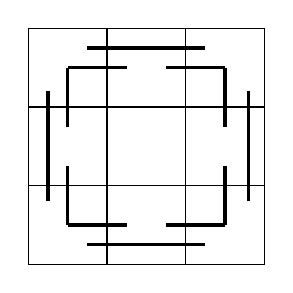
\begin{tikzpicture}
 \foreach \a/\b in { 0/0, 0/1, 0/2, 1/0, 1/1, 1/2, 2/0, 2/1, 2/2 } \draw (\a,\b) rectangle (\a+1,\b+1);
 \draw[very thick] ( 0.5, 0.50) -- (1.25, 0.50);
 \draw[very thick] ( 0.5, 0.50) -- ( 0.5, 1.25);
 \draw[very thick] (1.75, 0.50) -- (2.50, 0.50);
 \draw[very thick] (2.50, 0.50) -- (2.50, 1.25);
 \draw[very thick] ( 0.5, 1.75) -- ( 0.5, 2.50);
 \draw[very thick] ( 0.5, 2.50) -- (1.25, 2.50);
 \draw[very thick] (1.75, 2.50) -- (2.50, 2.50);
 \draw[very thick] (2.50, 2.50) -- (2.50, 1.75);

 \draw[very thick] (0.25, 0.80) -- (0.25, 2.20);
 \draw[very thick] (2.80, 0.80) -- (2.80, 2.20);

 \draw[very thick] (0.75, 2.75) -- (2.25, 2.75);
 \draw[very thick] (0.75, 0.25) -- (2.25, 0.25);
\end{tikzpicture}
\caption{\label{fig:gridnode} Attempt to transform $3 \times 3$ grid $G$ to a ring}
\end{figure}

Thus, since constructing a ring is already impossible for this specific grid $G$, it cannot be done in general as claimed.
\end{proof}

The previous lemma leads to an interesting observation: since a $3 \times 3$ grid $G$ cannot be transformed into a ring of $9$ edges, there cannot be a ring describing this specific $3 \times 3$ grid $G$. We obtain:
\\
\begin{corollary} \label{col:ring2grid}
Let $R$ be a ring containing $n * n$ edges. Then, there is no general way to transform $R$ to a grid of size $n \times n$.
\end{corollary}

From the two observations above, we conclude that we cannot use algorithms operating on ring networks. However, the study of ring networks is still useful to us: we can show that if leader election without unique identification numbers is not possible for ring networks, it cannot be done for grid networks either.
\\
\begin{theorem} \label{thm:needuid}
There is no deterministic algorithm $\mAA$ for leader election for any grid $G$ containing $n \times n$ edges if all nodes are completely identical.
\end{theorem}
\begin{proof}
Let us consider a grid $G$ of $2 \times 2$ nodes. Clearly, we can transform this grid to a ring as it is basically already a ring of $4$ edges. From \cite[Theorem 3.1]{lynch96distalgo} it follows that this problem cannot be solved without a way to distinguish the individual nodes, proving the theorem.
\end{proof}

Based on the hardware in use as outlined in Section \ref{sec:hardware}, we expect to have a pretty poor pseudo random generator. Based on this observation and Theorem \ref{thm:needuid}, it follows that the node identifiers are actually required. Fortunately, there is a unique identifier per node and we consequently use this identifier to elect a unique leader: the node with the lowest identifier becomes the leader. The following algorithm is proposed to carry out this procedure:

\begin{myalgo}{LeaderElection}{id}
 \qcomment{Initially, we believe we are the leader - but we haven't told anyone yet} \\
 $mustSend \qlet true$ \\
 $leaderid \qlet id$ \\
 \label{elect:loop} \qwhile leader election is in progress \\
 \label{elect:checksend} \qdo \qif $mustSend$ \\
  \qthen \qcomment{We haven't yet told who we believe the leader is} \\
         Send a message $(id, leaderid)$ to all directly connected nodes \\
         \label{elect:endsend} $mustSend \qlet false$ \qfi \\
  \label{elect:recv} \qif a message $(nodeid, newid)$ is received \\
  \qthen \qcomment{Someone believes he has new leader for us} \\
         \qif $newid < leaderid$ \\
         \qthen \qcomment{The proposed leader is better than the one we currently have} \\
                $leaderid \qlet newid$ \\
                \qcomment{Inform all our direct nodes about this new leader} \\
                \label{elect:recvdone} $mustSend \qlet true$ \\
         \qelse \label{elect:ign1} \qcomment{Our leader is better than what we received} \\
                \label{elect:ign2} \qignore \qfi \qfi \qelihw \\
  \label{elect:checkldr} \qcomment{We are done. If $id = leaderid$, we act as leader}
\end{myalgo}

First of all, line \ref{elect:loop} states that this algorithm should run while the leader election is in progress. This obviously begs the question: when is the leadership election done? The answer is that we cannot know - a leader does not keep an overview of all nodes, so it can't keep track of whether all nodes acknowledge their leader. And even if such a mechanism was to be implemented, if some node fails and never acknowledges the leader, we'd be waiting indefinitely. To prevent these issues, we say that the leader election phase ends if updates have not been received for 2 seconds. Even if the clock speed of all nodes may be off by a small percentage, the assumption is that messages are processed fast enough so that any lower identifier would have been received within this time.

By visual inspection of this rather straightforward algorithm, we expect it does the right thing: out of all nodes, the node with the lowest id becomes the leader. Since all id's are distinct, we know there is only one lowest id. Thus, a single node becomes the leader and all other nodes accept this course of action. However, can we provide a better founded argument? The algorithm will be described by means of a model in Chapter \ref{ch:leaderelection}, where it is proved that the necessary properties are satisfied.

\section{Coordinates determination}
\label{sec:opcoorddet}

Once a leader has been chosen, it must assign every node unique coordinates. The leader will consider itself to be at \coord{0,0} and in turn assign coordinates relative to this position to its neighboring nodes. However, nodes can be rotated any multiple of $90 \degree$, so it is important that all nodes in the network consider $0$ as the same direction, regardless of how each individual node is rotated. To this end, we must include the direction where the request should be received in the message, allowing the receiving node to determine how it is rotated and subsequently alter the meaning of its directions as needed. This results in all nodes assuming the rotation of the leader. Let us introduce how we can calculate the rotation based on the incoming and desired direction. Since all nodes are square-sized, they can be rotated $0 \degree, 90 \degree, 180 \degree$ and $270 \degree$. We shall introduce $r$ as a variable indicating the angle at which the node was rotated, where $rotation = r * 90 \degree$ to the right. The result is illustrated in Figure \ref{fig:rotations}.

\begin{figure}[h]
  \centering
  \begin{tikzpicture}
  \newcommand{\spnode}[6]{
   \draw (4*#1,0) rectangle (3+4*#1, 3);
   \draw (4*#1+1.5, 0.35) node {$#5$};
   \draw (4*#1+2.65,1.55) node {$#4$};
   \draw (4*#1+1.5, 2.65) node {$#3$};
   \draw (4*#1+0.35,1.55) node {$#6$};
   \draw (1.5+4*#1, -0.25) node {$r = #2$};
  }
   \foreach \a/\b/\c/\d/\e in { 0/0/1/2/3, 1/3/0/1/2, 2/2/3/0/1, 3/1/2/3/0 } \spnode{\a}{\a}{\b}{\c}{\d}{\e};
  \end{tikzpicture}
 \caption{\label{fig:rotations} Node rotation configurations, where $rotation = r * 90 \degree$}
\end{figure}

By looking at Figure \ref{fig:rotations}, we see that if an unrotated node ($r = 0$) is sending to direction $1$, a node with $r = 1$ would be sending to direction $0$, a node with $r = 2$ would be sending to direction $3$ and a node with $r = 3$ would be sending to direction $2$. There is a clear pattern here, which makes much more sense when we describe it: if some node $\mNN$ which is rotated $r$ turns to the right sends to direction $d$, this is the same as if an unrotated node would send to direction $d$ rotated $r$ turns to the left: the end result is the same.

By the above reasoning, we can define a rotate-left function, $rl(d,r) = (d - r) \mmod 4$: if the rotation is $r$ and the direction is $d$, the unrotated direction will be $d - r$, and since we have $4$ directions, we must perform the calculation modulo $4$. This function can also be used to find the actual rotation of a node: if we know the incoming direction $d$ and the expected direction $e$, we are interested in how much $d$ should be rotated to match $e$ - that is, we want to know what $e - d$ is, which is what $rl(e,d)$ calculates.

Once a node is aware of its rotation $r$, it can use this rotation to align its directions with the unrotated case. Let us consider an example: if a node has rotation $r = 2$ and it intends to send to unrotated direction $d = 1$, it should send to direction $3$, as illustrated in Figure \ref{fig:rotations}. As we have defined the rotation $r$ as the number of turns to the right, we can simply use output $(d + r) \mmod 4$ - this makes sense, as we are countering the left turns introduced by the $rl$ function. To this end, we appropriately introduce a rotate-right function $rr(d,r) = (d + r) \mmod 4$.

We need but one function: in order to determine the rotation of a node, we need the direction in which a message was received as well as the direction this message should have been received in. The first is available by means of the hardware (refer to Section \ref{sec:assumptions}), but the intended direction must be embedded in the message. Let us consider $r = 0$ in Figure \ref{fig:rotations}: if we send a message to direction $0$, we want it to be received in direction $2$. To this end, we can define a receiving-direction function $rd(i) = (i + 2) \mmod 4$.

Finally, we must define the coordinate system in use. To this end, we define the bottom-left coordinate as the lowest coordinate and subsequently, top-right is the highest coordinate in use. This is illustrated in Figure \ref{fig:relcoords}.

\begin{figure}[h]
\centering
\begin{nodefigure}
\nodegrid{3}{0}{0}{0/0/////, 1/0/\coord{ 0,-1}////, 2/0/////,
                   0/1/\coord{-1, 0}////, 1/1/\coord{0, 0}/$0$/$1$/$2$/$3$, 2/1/\coord{ 1, 0}////,
                   0/2/////, 1/2/\coord{ 0, 1}////, 2/2/////}
\end{nodefigure}
\caption{\label{fig:relcoords} Relative coordinates between nodes}
\end{figure}

Based on Figure \ref{fig:relcoords}, we can define a function $\Delta(c,d)$, which given a coordinate $c = \coord{x,y}$ and a direction $d$ returns the corresponding coordinate if coordinate $c$ is moved one position in direction $d$:

\begin{center}
\begin{tabular}{|l|l|}
\hline
\textbf{$d$} & \textbf{$\Delta(\coord{x,y}, d)$} \\
\hline
$0$     & $\coord{x,y+1}$ \\
\hline
$1$     & $\coord{x+1,y}$ \\
\hline
$2$     & $\coord{x,y-1}$ \\
\hline
$3$     & $\coord{x-1,y}$ \\
\hline
\end{tabular}
\end{center}

Using these definitions, we propose the following algorithm:

\begin{myalgo}{DetermineCoords}{id, actAsLeader}
 \qcomment{Initially, we always believe we are at \coord{0,0} and we are not rotated} \\
 $coord  \qlet \coord{0,0}$, $r \qlet 0$ \\
 \qcomment{The leader must initiate the procedure} \\
 $mustSend \qlet actAsLeader$ \\
 \qwhile coordinate determination is in progress \label{sp2:loop} \\
 \qdo \qcomment{Communicate new coordinates as necessary} \\
       \qif $mustSend$ \label{sp2:send1} \\
       \qthen \qcomment{Communicate coordinates to direction $i$} \\
              For all $0 \leq i \leq 3$: send coordinates $\Delta(coord, rr(i, r))$ using output $i$ \\
              where receiving direction should be $rr(rd(i), r)$ \\
              $mustSend \qlet false$ \qfi \label{sp2:send2} \\
      \qif a message $(newcoord, dir)$ has been received from direction $source$ \\
      \qthen \qif $coord = \coord{0, 0} \land \lnot actAsLeader$ \label{sp2:isinitial} \\
             \qthen \qcomment{We did not receive initial coordinates, so update them} \label{sp2:recinit1} \\
                    $coord \qlet newcoord$ \\
                    $r \qlet rl(dir, source)$  \\
                    \qcomment{We must inform our neighbors} \\
                    $mustSend \qlet true$ \qfi \label{sp2:recinit2} \\
             \qelse \qcomment{We already know our coordinates} \\ \label{sp2:recnext1}
                    \qif $coord \neq newcoord$ \\
                    \qthen \qcomment{We receive different coordinates - this indicates multiple leaders} \\
                           \label{sp2:rejectcoord} \qreset \\
                    \qelse \qcomment{Position is correct - check rotation} \\
                           \qif $rl(dir, source) \neq r$ \label{sp2:badrot} \\
                           \qthen \qcomment{Rotation is not correct} \\
                                  \qreset \\
                           \qelse \qcomment{We received the same coordinate on the correct input} \\
                                  \qignore \qfi \qfi \qfi \qfi \qelihw \label{sp2:recnext2}
\end{myalgo}

First of all, it must be noted that there are two approaches possible while sending updates in line \ref{sp2:send1} - \ref{sp2:send2}: we can either send to actual output pin $i$, regardless of its orientation or we can send to the pin that becomes output pin $i$ after countering the rotation. In our approach, we have chosen the first option as it makes the model clearer to understand and the second option doesn't provide any additional benefit.

The loop in line \ref{sp2:loop} has to terminate at some point - however, as before, we do not know when all nodes have been given coordinates as we do not know how many nodes there are. Thus, our only option is to continue to the next phase if we haven't received messages for a period of time, similar to leadership election.

Using the proposed algorithm, we note that once the rotation $r$ is calculated as $r = rl(d,n)$, we expect that sending a message back to $n$ using rotation $r$ by means of $rl(n,r)$ means we actually use direction $d$. This is proved in Lemma \ref{lemma:samedir}.
\\
\begin{lemma} \label{lemma:samedir} For any node number $n$ and direction $d$, it holds that $rr(n, rl(d,n)) = d$ \end{lemma}
\begin{proof}
\begin{derivation}{$rr(n, rl(d,n)) = d$}
\equ{Declaration $rr$}{$(n + rl(d,n)) \mmod 4 = d$}
\equ{Declaration $rl$}{$(n + ((d - n) \mmod 4)) \mmod 4 = d$}
\equ{Algebra}{$(n + d - n) \mmod 4 = d$}
\equ{Algebra}{$d \mmod 4 = d$}
\equ{$0 \leq d \leq 3$}{$true$}
\end{derivation}
\end{proof}

An interesting observation is that Lemma \ref{lemma:samedir} actually implies the condition in algorithm line \ref{sp2:badrot} cannot occur: if the leader sends a message from which the rotation is calculated, subsequent verification of the calculated rotation will always succeed. However, it is not specified whether nodes can be rotated without resetting them; if this behavior is possible, algorithm line \ref{sp2:badrot} can indeed occur and the result is that the system will reset itself as intended.

\section{Grid size determination}
\label{sec:opgridsize}

Once a node has entered this phase of the protocol, the node knows whether it is the leader, its coordinates within the grid and its rotation relative to the leader. However, the size of the grid is not known, while it is needed in order to determine which light should be switched on/off to display the intended figure. To this end, the grid size determination algorithm is run: each node communicates its maximal and minimal coordinates to its neighbors, which compare these coordinates to their current minimal and maximal coordinates. If this results in better (i.e. smaller minimum or greater maximum) coordinates, the node will update their current coordinates and communicate these to all adjacent nodes. The desired result is that every node learns the minimal and maximal coordinates in this grid, from which the total grid size can be derived.

First of all, we have to determine how coordinates are compared: when is one coordinate smaller or greater than another coordinate? In order to do this, keep in mind that we are looking for the bottom-left and top-right coordinates. In other words, coordinates $\coord{x_1, y_1} \leq \coord{x_2, y_2}$ if $x_1 \leq x_2$ and $y_1 \leq y_2$. The same goes for the maximum coordinates: $\coord{x_1, y_1} \geq \coord{x_2, y_2}$ if $x_1 \geq x_2$ and $y_1 \geq y_2$. This means the minimum of two coordinates are their smallest $x$ and $y$ values, whereas the maximum of two $x$ and $y$ values are their largest $x$ and $y$ values. Thus, $\mmin(\coord{x_1, y_1}, \coord{x_2, y_2}) = \coord{\mmin(x_1,x_2), \mmin(y_1,y_2)}$ and $\mmax(\coord{x_1, y_1}, \coord{x_2, y_2}) = \coord{\mmax(x_1,x_2), \mmax(y_1,y_2)}$.

Using these declarations, we propose the following algorithm to perform these actions:

\begin{myalgo}{DetermineGridSize}{id, actAsLeader, leaderid, coord}
 \qcomment{Initially, we believe our own coordinates are both the minimum and maximum} \\
 $minCoord, maxCoord \qlet coord, coord$ \\
 \qcomment{If we are leader, initiate the procedure. Otherwise, just wait} \\
 $mustSend \qlet actAsLeader$ \\
 \qwhile grid size determination is in progress \label{sp3:loopcond} \\
 \qdo \qcomment{Communicate new min/max coordinates as necessary} \\
       \qif $mustSend$ \label{sp3:sent1} \\
       \qthen \qcomment{Broadcast the min/max coordinates} \\
              Send $(leaderid, minCoord, maxCoord)$ to all outputs \\
              $mustSend \qlet false$ \qfi \label{sp3:sent2} \\
      \qif a message $(lid, minc, maxc)$ has been received \\
      \qthen \qcomment{Received a new message - check consistency} \\
             \qif $lid > leaderid$ \label{sp3:multil1} \\
             \qthen \qcomment{There are multiple leaders!} \\
                    \qreset \qfi \label{sp3:multil2} \\
             \qif $minc < minCoord$ \qor $maxc > maxCoord$ \\
             \qthen \qcomment{We have obtained smaller minimal or greater maximal coordinates} \label{sp3:new1}\\
                    $minCoord \qlet \mmin(minc,minCoord)$ \\
                    $maxCoord \qlet \mmax(maxc,maxCoord)$ \\
                    \qcomment{Update our leader id; $lid$ can only be less or equal to} \\
                    \qcomment{the current leader id} \\
                    $leaderid \qlet lid$ \\
                    \qcomment{Inform our neighbors about this} \\
                    $mustSend \qlet true$ \label{sp3:new2} \\
             \qelse \qcomment{We have a clearer picture of our grid than our neighbor. Yet, } \\
                    \qcomment{we may have received an even lower leader id so honor it} \\
                    $leaderid \qlet lid$ \qfi \label{sp3:ignore} \qelihw
\end{myalgo}

As usual, we should define what the condition in line \ref{sp3:loopcond} is: just looping forever waiting for new coordinates that never arrive can hardly be considered productive. However, like during the leader election, we cannot know if we have received the `correct' minimum/maximum coordinates, since each node cannot know what the network's minimum/maximum coordinate is - this is why we introduced this phase to begin with! Thus, all we can do is wait until we have not received updates for a certain period of time and assume the maximum coordinates has been received by then, similar to what we do in the leadership election phase.

\section{Showtime}

During this phase, all necessary information has been acquired: each node knows who the leader is, its coordinates within the grid and rotation relative to the leader and finally, the size of the grid in use. The only remaining part is that nodes should display the desired figures; these actions are initiated by the leader node. We assume that upon power-on, the light is switched off, since there is too little information available to start displaying a figure.

The following algorithm is proposed:

\begin{myalgo}{Showtime}{id, actAsLeader, leaderid,lpos,mincoord,maxcoord}
 \qwhile true \\
 \qdo \qcomment{The leader is responsible for initiating activity} \\
      \qif $actAsLeader$ \qand 2 seconds have elapsed \\
      \qthen \qcomment{The time has come} \\
	     $figure \qlet (figure +1 ) \mmod 2$ \label{sp4:timer1} \\
             Update light to confirm to $figure$ \\
             Send a message $(id,figure)$ to all directly connected nodes \label{sp4:timer2} \qfi \\
      \qif a message $(lid, newfigure)$ has been received \\
      \qthen \qif $lid > leaderid$ \\
             \qthen \qcomment{Someone else is pretending to be our leader} \\
                    \qreset \label{sp4:leadererr} \\
             \qelse \qif $figure \neq newfigure$ \\
                    \qthen \qcomment{Follow the leader} \\
                           $figure \qlet newfigure$ \label{sp4:sendfollow} \\
                           Update light to confirm to $newfigure$ \\
                           \qcomment{We may have received an even lower leader id, so honor it} \\
                           $leaderid \qlet lid$ \\
                           Send a message $(leaderid, newfigure)$ to all directly connected nodes \label{sp4:send2}\\
                    \qelse \qcomment{Our current status is fine, but the leader id may be lower} \\
                           $leaderid \qlet lid$ \label{sp4:ignupdate} \qfi \qfi \qelihw
\end{myalgo}

We note that we need a function which, given a node's coordinates, the minimal/maximal node coordinate and the figure that needs to be displayed determines whether the light should be switched on or off. We shall first give a specification for figures $0$ and $1$ as illustrated in Figure \ref{fig:showtimefig}.

\begin{figure}[h]
 \centering
 \begin{tikzpicture}
  \newcommand{\fillnode}[2]{\draw[fill] (0.75*#1,0.75*#2) rectangle (0.75+0.75*#1,0.75+0.75*#2);}
  \draw[step=0.75cm] (0, 0) grid (3.75,3.75);
  \foreach \a/\b in {
    1/0, 2/0, 3/0,
    0/1, 0/2, 0/3,
    4/1, 4/2, 4/3,
    1/4, 2/4, 3/4
  } \fillnode{\a}{\b};
  \renewcommand{\fillnode}[2]{\draw[fill] (5.245+0.75*#1,0.75*#2) rectangle (5.995+0.75*#1,0.75+0.75*#2);}
  \draw (1.875, -0.25) node {$n = 0$};
  \draw[step=0.75cm] (5.245, 0) grid (9,3.75);
  \foreach \a/\b in {
   0/0, 1/1, 2/2, 3/3, 4/4,
   0/4, 1/3,      3/1, 4/0
  } \fillnode{\a}{\b};
  \draw (6.875, -0.25) node {$n = 1$};
 \end{tikzpicture}
 \caption{\label{fig:showtimefig} Figures displayable by the nodes}
\end{figure}

The circular figure, $n = 0$, can be shown by lighting only the nodes at the border, with the exception of the nodes at the far edges. This gives the following formula:

\begin{tabbing}
\hspace{2cm} \= \\
$light(\coord{node_x,node_y}, \coord{min_x,min_y}, \coord{max_x,max_y}, \mbox{circle}) =$ \\
\> $(node_x = min_x \lor node_x = max_x \lor node_y = min_y \lor node_y = max_y)~\land$ \\
\> $\coord{node_x, node_y} \not\in \{ \coord{min_x, min_y}, \coord{max_x, min_y}, \coord{min_x, max_y}, \coord{max_x, max_y}$ \} \\
\end{tabbing}

As for the cross, determining the light state is a bit more involved. First of all, we want to normalize the grid coordinates, so that coordinate \coord{0,0} is the bottom-left. This is illustrated in Figure \ref{fig:coordnoorm}. Note that $min = \coord{-2, -1}$ and $max = \coord{0, 1}$ - to this end, we need to subtract $min$ from all coordinates.

\begin{figure}[h]
\centering
\begin{nodefigure}
\nodegrid{3}{0}{0}{0/0/\coord{-2,-1}////, 1/0/\coord{-1,-1}////, 2/0/\coord{ 0,-1}////,
                   0/1/\coord{-2, 0}////, 1/1/\coord{-1, 0}////, 2/1/\coord{ 0, 0}////,
                   0/2/\coord{-2, 1}////, 1/2/\coord{-1, 1}////, 2/2/\coord{ 0, 1}////}
\nodegrid{3}{4}{0}{0/0/\coord{ 0, 0}////, 1/0/\coord{ 1, 0}////, 2/0/\coord{ 2, 0}////,
                   0/1/\coord{ 0, 1}////, 1/1/\coord{ 1, 1}////, 2/1/\coord{ 2, 1}////,
                   0/2/\coord{ 0, 2}////, 1/2/\coord{ 1, 2}////, 2/2/\coord{ 2, 2}////}
\draw[->,>= stealth'] ( 5, 2.25) -- (5.5, 2.25);
\end{nodefigure}
\caption{\label{fig:coordnoorm} Coordinate normalization: bottom-left becomes \coord{0,0}}
\end{figure}

Now, we note that the bottom-left to top-right diagonal is simply determining whether the $x$ and $y$ coordinates are equal. The top-left to bottom-right coordinate means that the sum of the $x$ and $y$ coordinate is a fixed value: namely, the dimension of the grid minus 1. This gives the following formula:

\begin{tabbing}
\hspace{2cm} \= \\
$light(\coord{node_x,node_y}, \coord{min_x,min_y}, \coord{max_x,max_y}, \mbox{cross}) =$ \\
\> $x = y~\lor$ \\
\> $x + y = d$ \\
\textbf{where} \> $\coord{x,y} = \coord{node_x - min_x, node_y - min_y}$ \\
               \> $d = max_x - min_x$ \\
\end{tabbing}

\section{Resetting the system}
\label{sec:reset}

The previous algorithms all rely on a \TT{reset} action, which serves the purpose of instructing the complete node network to reset itself as something is flawed. Obviously, we need to describe this operation as we definitely do not intend to reset the system forever. To this end, upon power-on, a node must initialize $mustReset = false$ and $resetcount = 0$.

\begin{myalgo}{ResetAlgorithm}{}
\qwhile $true$ \\
  \qif $mustReset$ \\
  \qthen \qcomment{We haven't sent our reset to our neighbors yet} \\
         Send a message $resetcount$ to all directly connected nodes \\
         \qcomment{Increment the reset count, to ensure we do not honor this reset again} \\
         $resetcount \qlet (resetcount + 1) \mmod 10$ \\
         \label{reset:doit} Reset our current node \qfi \\
  \label{reset:recv} \qif a message $count$ is received \\
  \qthen \qcomment{We might have to reset} \\
         \qif $count \geq resetcount$ \\
         \qthen \qcomment{We must be resetting} \\
                $mustReset \qlet true$ \\
         \qelse \qcomment{We have already honored this reset round} \\
                \qignore \qfi \qfi \qelihw
\end{myalgo}

As can be seen, the $ResetAlgorithm$ algorithm runs forever - this is because the algorithm should always be active, as reset messages must be processed in any state of the system: $ResetAlgorithm$ must always run in parallel with the current algorithm in the system. Furthermore, the result of the \TT{reset} actions is that $mustReset$ should be set to $true$.

The actual reset performed in line \ref{reset:doit} should perform a reinitialization of the node. Specifically, the node should start in leader election phase, while $mustReset$ is set to $false$. The $resetcount$ value must not be changed, as this value is used to keep the network from resetting indefinitely.

\section{Research questions}
\label{sec:questions}

We will describe several research questions which will be answered in this thesis:

\begin{enumerate}
\item The system sketch describes distinct system modes and transitions between these modes. What is the system behavior if these modes are merged, i.e. any message can arrive in any mode? \\
This question is discussed in Sections \ref{sec:ignoreoop} to \ref{sec:ignorephase}.
\item Does the network adapt correctly if nodes are added or removed from the system? \\
This question is discussed in Section \ref{sec:alteringconfig}.
\item Can we determine how long a node should wait before electing itself as leader? \\
This question is discussed in Section \ref{sec:timedle}.
\item What happens if messages are not guaranteed to arrive? \\
This question is discussed in Section \ref{sec:unreliablecomm}.
\end{enumerate}

We will begin by proving correctness of the algorithms in a fixed configuration, under ideal circumstances: messages always arrive and the node configuration is never changed. The goal is to determine whether the algorithms we have presented are correct at all. In Chapter \ref{ch:overallsystem}, the influence of unreliable communication and adding/removing nodes will be discussed.

Chapters \ref{ch:leaderelection} to \ref{ch:showtime} all discuss the following $3 \times 3$ grid configuration:

\begin{figure}[h]
\centering
\begin{nodefigure}
\nodegrid{3}{0}{0}{0/2/0/$0$/$1$/$2$/$3$, 1/2/1/$1$/$2$/$3$/$0$, 2/2/2/$2$/$3$/$0$/$1$,
                   0/1/3/$3$/$0$/$1$/$2$, 1/1/4/$3$/$0$/$1$/$2$, 2/1/5/$0$/$1$/$2$/$3$,
                   0/0/6/$1$/$2$/$3$/$0$, 1/0/7/$0$/$1$/$2$/$3$, 2/0/8/$2$/$3$/$0$/$1$}
\end{nodefigure}
\caption{\label{fig:configused} The $3 \times 3$ node configuration used during the analysis in chapters \ref{ch:leaderelection} to \ref{ch:showtime}}
\end{figure}

Unfortunately, it is not possible to model an arbitrary configuration, as the statespace tends to grow so large in such situations that it is no longer manageable. Fortunately, a $3 \times 3$ grid seems sufficient to determine problems within the system; after completing the analysis of a $3 \times 3$ grid, an attempt has been made to analyze a $4 \times 4$ grid. The results were that even though the analysis took much longer, it did not yield any different results. This leads us to believe that analyzing a $3 \times 3$ grid is sufficient as it already illustrates any potential problems.
